\documentclass[9pt]{beamer}

% Beamer style
%\usetheme[secheader]{Madrid}
% \usetheme{CambridgeUS}
\useoutertheme{infolines}
\usecolortheme[rgb={0.65,0.15,0.25}]{structure}
% \usefonttheme[onlymath]{serif}
\beamertemplatenavigationsymbolsempty
%\AtBeginSubsection

% Packages
%\usepackage[french]{babel}
\usepackage[latin1]{inputenc}
\usepackage{color}
\usepackage{xspace}
\usepackage{dsfont, stmaryrd}
\usepackage{amsmath, amsfonts, amssymb, stmaryrd}
\usepackage{epsfig}
\usepackage{tikz}
\usepackage{url}
% \usepackage{ulem}
\usepackage{/home/robin/LATEX/Biblio/astats}
%\usepackage[all]{xy}
\usepackage{graphicx}
\usepackage{xspace}

\input{/home/robin/RECHERCHE/EXPOSES/LATEX/Commands}

% Directory
\newcommand{\fignet}{/home/robin/Bureau/RECHERCHE/RESEAUX/EXPOSES/FIGURES}
\newcommand{\figtree}{/home/robin/RECHERCHE/BAYES/VBEM-IS/VBEM-IS.git/Data/Tree/Fig}

%====================================================================
%====================================================================

%====================================================================
%====================================================================
\begin{document}
%====================================================================
%====================================================================

%====================================================================
\title{The stochastic block-model and its (variational) inference}

\author{S. Robin}

\institute[INRA/AgroParisTech/Paris-Saclay]{INRA / AgroParisTech /univ. Paris-Saclay}

\date[Stat. Math., IHP]{3�me journ�e du groupe Statistique Math�matique de la SFdS \\ ~\\ 
  Graphes al�atoires et Statistique \\ ~\\
  Paris, IHP, Janvier 2019}

%====================================================================
%====================================================================
\maketitle
%====================================================================

%====================================================================
\frame{\frametitle{Karate club}

  $n = 34$ nodes (individuals), link = mutual friendship
  $$
  \includegraphics[height=.6\textheight, width=.4\textwidth]{\fignet/Karate-Graph1}
  \qquad \pause
  \includegraphics[height=.6\textheight, width=.4\textwidth]{\fignet/Karate-Graph2}
  $$
}

%====================================================================
\frame{\frametitle{Tree ecological network}

\begin{itemize}
 \item $n = 51$ tree species, 
 \item $Y_{ij} =$ number of shared parasites, 
 \item $x_{ij} =$ (taxonomic, geographic, genetic distances)
\end{itemize}

\begin{tabular}{cc}
 \begin{tabular}{p{.5\textwidth}}
  \onslide+<2->{Without covariates: $\Pcal(e^{\gamma_{k\ell}})$ \\
  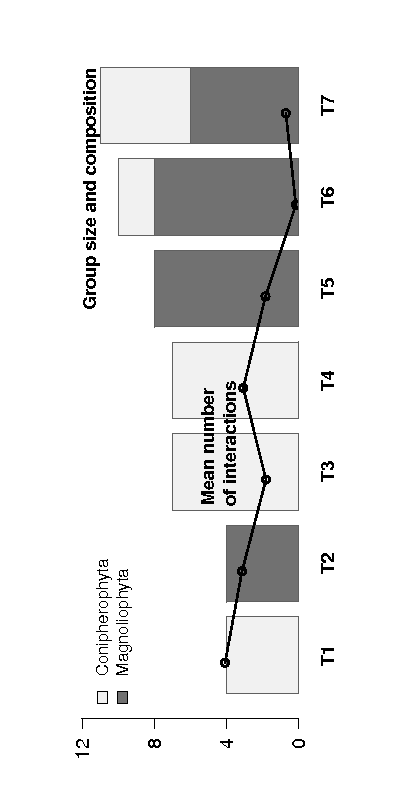
\includegraphics[height=.65\textheight, width=.35\textwidth, angle=270]{\fignet/MRV10_AoAS_Q7_group}
  }
  \end{tabular}
  & 
  \hspace{-.05\textwidth}
  \begin{tabular}{p{.5\textwidth}}
  \onslide+<3->{With covariates: $\Pcal(e^{\gamma_{k\ell} + x_{ij}^\trans \beta})$ \\
  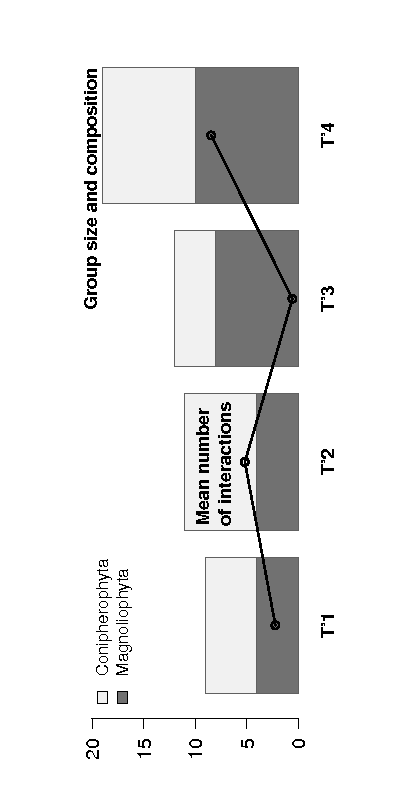
\includegraphics[height=.6\textheight, width=.35\textwidth, angle=270]{\fignet/MRV10_AoAS_Q4_group}
  }
 \end{tabular}
\end{tabular}

\footnotesize{Mariadassou \& al., Ann. Applied Stat., 2010}

}

%====================================================================
\frame{\frametitle{Onager network}

$n = 23$ individuals, $T = 4$ dates, $\widehat{K} = 4$ groups

$$
\includegraphics[height=.5\textheight, width=.8\textwidth]{\fignet/MaM17-JRSSB-Fig8b}
$$
\footnotesize{Matias \& Miele, JRSSB, 2017}

}


%====================================================================
\frame{\frametitle{$W$-graph}

  \begin{tabular}{cc}
	\onslide+<1->{
	\begin{tabular}{p{.5\textwidth}}
	\paragraph{A graphon function: $w(u, u')$.} ~ \\
	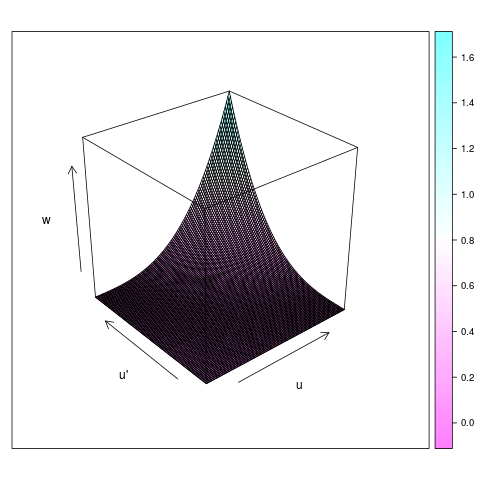
\includegraphics[width=.4\textwidth]{../FIGURES/FigCLADAG-W-graphon2} 
	\end{tabular}
	} 
    & 
    \hspace{-.1\textwidth}
	\onslide+<2->{
	\begin{tabular}{p{.5\textwidth}}
	\paragraph{Graphon function of an SBM.} ~ \\
	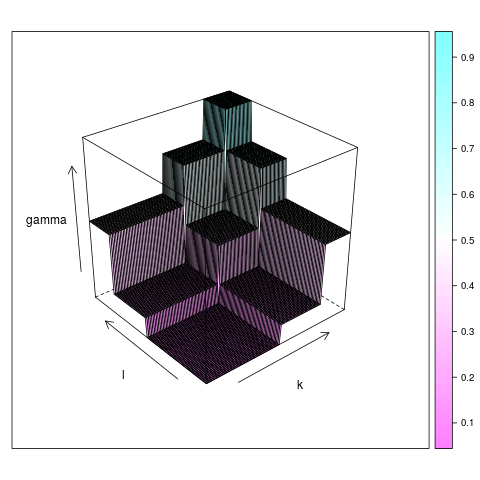
\includegraphics[width=.4\textwidth]{../FIGURES/FigCLADAG-SBM-graphon} 
	\end{tabular}
	}
  \end{tabular}

}


%====================================================================
\frame{\frametitle{Graphical models (Lauritzen, 96)}

\paragraph{Directed graphical models:} $p$ faithfull to $G$ (DAG) iff
$$
p(U_1, \dots U_m) = \prod_j p(U_j \mid U_{pa_G(j)})
$$
where $U_J = \{U_j: j \in J\}$ and $pa_G(j) =$ sets of parents of $j$ in $G$.

\bigskip \bigskip \bigskip \pause
\paragraph{Undirected graphical models:} $p$ faithfull to $G$ iff
$$
p(U_1, \dots U_m) \propto \prod_{C \in \Ccal(G)} \Psi_C(U_C)
$$
where $\Ccal(G) =$ set of all maximal cliques of $G$.

\bigskip \bigskip 
\begin{itemize}
\item Directed GM $\rightarrow$ Undirected GM, via moralization.
\item Undirected GM: Equivalence between separation and conditional independence.
\end{itemize}
}

%====================================================================
\frame{\frametitle{Graphical models for the dynamic SBM}

  \begin{overprint}
  \onslide<1>
  \paragraph{Hidden Markov chains.} $n = 3$, $T = 3$~ \\
  $$
  \begin{tikzpicture}
  \node[hidden] (Z11) at (0, 2*\edgeunit) {$Z_1^1$};
  \node[hidden] (Z21) at (-.5*\edgeunit, \edgeunit) {$Z_2^1$};
  \node[hidden] (Z31) at (0, 0) {$Z_3^1$};

  \node[hidden] (Z12) at (2*\edgeunit, 2*\edgeunit) {$Z_1^2$};
  \node[hidden] (Z22) at (1.5*\edgeunit, \edgeunit) {$Z_2^2$};
  \node[hidden] (Z32) at (2*\edgeunit, 0) {$Z_3^2$};

  \node[hidden] (Z13) at (4*\edgeunit, 2*\edgeunit) {$Z_1^3$};
  \node[hidden] (Z23) at (3.5*\edgeunit, \edgeunit) {$Z_2^3$};
  \node[hidden] (Z33) at (4*\edgeunit, 0) {$Z_3^3$};
  
  \node[blank] (Y121) at (.75*\edgeunit, 1.75*\edgeunit) {$Y_{12}^1$};
  \node[blank] (Y131) at (.5*\edgeunit, 1.25*\edgeunit) {$Y_{13}^1$};
  \node[blank] (Y231) at (.75*\edgeunit, .25*\edgeunit) {$Y_{23}^1$};
  
  \node[blank] (Y122) at (2.75*\edgeunit, 1.75*\edgeunit) {$Y_{12}^2$};
  \node[blank] (Y132) at (2.5*\edgeunit, 1.25*\edgeunit) {$Y_{13}^2$};
  \node[blank] (Y232) at (2.75*\edgeunit, .25*\edgeunit) {$Y_{23}^2$};
  
  \node[blank] (Y123) at (4.75*\edgeunit, 1.75*\edgeunit) {$Y_{12}^3$};
  \node[blank] (Y133) at (4.5*\edgeunit, 1.25*\edgeunit) {$Y_{13}^3$};
  \node[blank] (Y233) at (4.75*\edgeunit, .25*\edgeunit) {$Y_{23}^3$};

  \draw[arrow] (Z11) to (Z12);  \draw[arrow] (Z12) to (Z13);
  \draw[arrow] (Z21) to (Z22);  \draw[arrow] (Z22) to (Z23);
  \draw[arrow] (Z31) to (Z32);  \draw[arrow] (Z32) to (Z33);
  
  \end{tikzpicture}
  $$
  \onslide<2>
  \paragraph{Observed network at $t=1$.} \\
  $$
  \begin{tikzpicture}
  \node[hidden] (Z11) at (0, 2*\edgeunit) {$Z_1^1$};
  \node[hidden] (Z21) at (-.5*\edgeunit, \edgeunit) {$Z_2^1$};
  \node[hidden] (Z31) at (0, 0) {$Z_3^1$};

  \node[hidden] (Z12) at (2*\edgeunit, 2*\edgeunit) {$Z_1^2$};
  \node[hidden] (Z22) at (1.5*\edgeunit, \edgeunit) {$Z_2^2$};
  \node[hidden] (Z32) at (2*\edgeunit, 0) {$Z_3^2$};

  \node[hidden] (Z13) at (4*\edgeunit, 2*\edgeunit) {$Z_1^3$};
  \node[hidden] (Z23) at (3.5*\edgeunit, \edgeunit) {$Z_2^3$};
  \node[hidden] (Z33) at (4*\edgeunit, 0) {$Z_3^3$};

  \node[observed] (Y121) at (.75*\edgeunit, 1.75*\edgeunit) {$Y_{12}^1$};
  \node[observed] (Y131) at (.5*\edgeunit, 1.25*\edgeunit) {$Y_{13}^1$};
  \node[observed] (Y231) at (.75*\edgeunit, .25*\edgeunit) {$Y_{23}^1$};
  
  \node[blank] (Y122) at (2.75*\edgeunit, 1.75*\edgeunit) {$Y_{12}^2$};
  \node[blank] (Y132) at (2.5*\edgeunit, 1.25*\edgeunit) {$Y_{13}^2$};
  \node[blank] (Y232) at (2.75*\edgeunit, .25*\edgeunit) {$Y_{23}^2$};
  
  \node[blank] (Y123) at (4.75*\edgeunit, 1.75*\edgeunit) {$Y_{12}^3$};
  \node[blank] (Y133) at (4.5*\edgeunit, 1.25*\edgeunit) {$Y_{13}^3$};
  \node[blank] (Y233) at (4.75*\edgeunit, .25*\edgeunit) {$Y_{23}^3$};

  \draw[arrow] (Z11) to (Z12);  \draw[arrow] (Z12) to (Z13);
  \draw[arrow] (Z21) to (Z22);  \draw[arrow] (Z22) to (Z23);
  \draw[arrow] (Z31) to (Z32);  \draw[arrow] (Z32) to (Z33);
  
  \draw[arrow] (Z11) to (Y121);  \draw[arrow] (Z21) to (Y121);
  \draw[arrow] (Z11) to (Y131);  \draw[arrow] (Z31) to (Y131);
  \draw[arrow] (Z21) to (Y231);  \draw[arrow] (Z31) to (Y231);
  
  \end{tikzpicture}
  $$
  \onslide<3>
  \paragraph{Observed networks at $t = 1, \dots T$.} ~ \\
  $$
  \begin{tikzpicture}
  \node[hidden] (Z11) at (0, 2*\edgeunit) {$Z_1^1$};
  \node[hidden] (Z21) at (-.5*\edgeunit, \edgeunit) {$Z_2^1$};
  \node[hidden] (Z31) at (0, 0) {$Z_3^1$};

  \node[hidden] (Z12) at (2*\edgeunit, 2*\edgeunit) {$Z_1^2$};
  \node[hidden] (Z22) at (1.5*\edgeunit, \edgeunit) {$Z_2^2$};
  \node[hidden] (Z32) at (2*\edgeunit, 0) {$Z_3^2$};

  \node[hidden] (Z13) at (4*\edgeunit, 2*\edgeunit) {$Z_1^3$};
  \node[hidden] (Z23) at (3.5*\edgeunit, \edgeunit) {$Z_2^3$};
  \node[hidden] (Z33) at (4*\edgeunit, 0) {$Z_3^3$};

  \node[observed] (Y121) at (.75*\edgeunit, 1.75*\edgeunit) {$Y_{12}^1$};
  \node[observed] (Y131) at (.5*\edgeunit, 1.25*\edgeunit) {$Y_{13}^1$};
  \node[observed] (Y231) at (.75*\edgeunit, .25*\edgeunit) {$Y_{23}^1$};
  
  \node[observed] (Y122) at (2.75*\edgeunit, 1.75*\edgeunit) {$Y_{12}^2$};
  \node[observed] (Y132) at (2.5*\edgeunit, 1.25*\edgeunit) {$Y_{13}^2$};
  \node[observed] (Y232) at (2.75*\edgeunit, .25*\edgeunit) {$Y_{23}^2$};
  
  \node[observed] (Y123) at (4.75*\edgeunit, 1.75*\edgeunit) {$Y_{12}^3$};
  \node[observed] (Y133) at (4.5*\edgeunit, 1.25*\edgeunit) {$Y_{13}^3$};
  \node[observed] (Y233) at (4.75*\edgeunit, .25*\edgeunit) {$Y_{23}^3$};

  \draw[arrow] (Z11) to (Z12);  \draw[arrow] (Z12) to (Z13);
  \draw[arrow] (Z21) to (Z22);  \draw[arrow] (Z22) to (Z23);
  \draw[arrow] (Z31) to (Z32);  \draw[arrow] (Z32) to (Z33);
  
  \draw[arrow] (Z11) to (Y121);  \draw[arrow] (Z21) to (Y121);
  \draw[arrow] (Z11) to (Y131);  \draw[arrow] (Z31) to (Y131);
  \draw[arrow] (Z21) to (Y231);  \draw[arrow] (Z31) to (Y231);
  
  \draw[arrow] (Z12) to (Y122);  \draw[arrow] (Z22) to (Y122);
  \draw[arrow] (Z12) to (Y132);  \draw[arrow] (Z32) to (Y132);
  \draw[arrow] (Z22) to (Y232);  \draw[arrow] (Z32) to (Y232);
  
  \draw[arrow] (Z13) to (Y123);  \draw[arrow] (Z23) to (Y123);
  \draw[arrow] (Z13) to (Y133);  \draw[arrow] (Z33) to (Y133);
  \draw[arrow] (Z23) to (Y233);  \draw[arrow] (Z33) to (Y233);
  
  \end{tikzpicture}
  $$
  \ra $(Z^t, Y^t)_t \sim HMM$ with $K^n$ states.
%   $$
%   \begin{tikzpicture}
%   \node[hidden] (Z1) at (0, .75*\edgeunit) {$Z^1$};
%   \node[hidden] (Z2) at (2*\edgeunit, .75*\edgeunit) {$Z^2$};
%   \node[hidden] (Z3) at (4*\edgeunit, .75*\edgeunit) {$Z^3$};
% 
%   \node[observed] (Y1) at (0*\edgeunit, 0*\edgeunit) {$Y_{12}^1$};
%   \node[observed] (Y2) at (2*\edgeunit, 0*\edgeunit) {$Y_{12}^2$};
%   \node[observed] (Y3) at (4*\edgeunit, 0*\edgeunit) {$Y_{12}^3$};
% 
%   \draw[arrow] (Z1) to (Z2);  \draw[arrow] (Z2) to (Z3);
%   
%   \draw[arrow] (Z1) to (Y1);  \draw[arrow] (Z2) to (Y2);  \draw[arrow] (Z3) to (Y3);
%   
%   \end{tikzpicture}
%   $$  
  \onslide<4>
  \paragraph{Graph moralization.} ~ \\
  $$
  \begin{tikzpicture}
  \node[hidden] (Z11) at (0, 2*\edgeunit) {$Z_1^1$};
  \node[hidden] (Z21) at (-.5*\edgeunit, \edgeunit) {$Z_2^1$};
  \node[hidden] (Z31) at (0, 0) {$Z_3^1$};

  \node[hidden] (Z12) at (2*\edgeunit, 2*\edgeunit) {$Z_1^2$};
  \node[hidden] (Z22) at (1.5*\edgeunit, \edgeunit) {$Z_2^2$};
  \node[hidden] (Z32) at (2*\edgeunit, 0) {$Z_3^2$};

  \node[hidden] (Z13) at (4*\edgeunit, 2*\edgeunit) {$Z_1^3$};
  \node[hidden] (Z23) at (3.5*\edgeunit, \edgeunit) {$Z_2^3$};
  \node[hidden] (Z33) at (4*\edgeunit, 0) {$Z_3^3$};

  \node[observed] (Y121) at (.75*\edgeunit, 1.75*\edgeunit) {$Y_{12}^1$};
  \node[observed] (Y131) at (.5*\edgeunit, 1.25*\edgeunit) {$Y_{13}^1$};
  \node[observed] (Y231) at (.75*\edgeunit, .25*\edgeunit) {$Y_{23}^1$};
  
  \node[observed] (Y122) at (2.75*\edgeunit, 1.75*\edgeunit) {$Y_{12}^2$};
  \node[observed] (Y132) at (2.5*\edgeunit, 1.25*\edgeunit) {$Y_{13}^2$};
  \node[observed] (Y232) at (2.75*\edgeunit, .25*\edgeunit) {$Y_{23}^2$};
  
  \node[observed] (Y123) at (4.75*\edgeunit, 1.75*\edgeunit) {$Y_{12}^3$};
  \node[observed] (Y133) at (4.5*\edgeunit, 1.25*\edgeunit) {$Y_{13}^3$};
  \node[observed] (Y233) at (4.75*\edgeunit, .25*\edgeunit) {$Y_{23}^3$};

  \draw[edge] (Z11) to (Z12);  \draw[edge] (Z12) to (Z13);
  \draw[edge] (Z21) to (Z22);  \draw[edge] (Z22) to (Z23);
  \draw[edge] (Z31) to (Z32);  \draw[edge] (Z32) to (Z33);
  
  \draw[edge] (Z11) to (Z21); \draw[edge] (Z11) to (Z31); \draw[edge] (Z21) to (Z31);
  \draw[edge] (Z12) to (Z22); \draw[edge] (Z12) to (Z32); \draw[edge] (Z22) to (Z32);
  \draw[edge] (Z13) to (Z23); \draw[edge] (Z13) to (Z33); \draw[edge] (Z23) to (Z33);
  
  \draw[edge] (Z11) to (Y121);  \draw[edge] (Z21) to (Y121);
  \draw[edge] (Z11) to (Y131);  \draw[edge] (Z31) to (Y131);
  \draw[edge] (Z21) to (Y231);  \draw[edge] (Z31) to (Y231);
  
  \draw[edge] (Z12) to (Y122);  \draw[edge] (Z22) to (Y122);
  \draw[edge] (Z12) to (Y132);  \draw[edge] (Z32) to (Y132);
  \draw[edge] (Z22) to (Y232);  \draw[edge] (Z32) to (Y232);
  
  \draw[edge] (Z13) to (Y123);  \draw[edge] (Z23) to (Y123);
  \draw[edge] (Z13) to (Y133);  \draw[edge] (Z33) to (Y133);
  \draw[edge] (Z23) to (Y233);  \draw[edge] (Z33) to (Y233);
  
  \end{tikzpicture}
  $$
  \onslide<5>
  \paragraph{Graphical model of $p(Z \mid Y)$.} ~ \\
  $$
  \begin{tikzpicture}
  \node[hidden] (Z11) at (0, 2*\edgeunit) {$Z_1^1$};
  \node[hidden] (Z21) at (-.5*\edgeunit, \edgeunit) {$Z_2^1$};
  \node[hidden] (Z31) at (0, 0) {$Z_3^1$};

  \node[hidden] (Z12) at (2*\edgeunit, 2*\edgeunit) {$Z_1^2$};
  \node[hidden] (Z22) at (1.5*\edgeunit, \edgeunit) {$Z_2^2$};
  \node[hidden] (Z32) at (2*\edgeunit, 0) {$Z_3^2$};

  \node[hidden] (Z13) at (4*\edgeunit, 2*\edgeunit) {$Z_1^3$};
  \node[hidden] (Z23) at (3.5*\edgeunit, \edgeunit) {$Z_2^3$};
  \node[hidden] (Z33) at (4*\edgeunit, 0) {$Z_3^3$};

  \node[blank] (Y121) at (.75*\edgeunit, 1.75*\edgeunit) {$Y_{12}^1$};
  \node[blank] (Y131) at (.5*\edgeunit, 1.25*\edgeunit) {$Y_{13}^1$};
  \node[blank] (Y231) at (.75*\edgeunit, .25*\edgeunit) {$Y_{23}^1$};
  
  \node[blank] (Y122) at (2.75*\edgeunit, 1.75*\edgeunit) {$Y_{12}^2$};
  \node[blank] (Y132) at (2.5*\edgeunit, 1.25*\edgeunit) {$Y_{13}^2$};
  \node[blank] (Y232) at (2.75*\edgeunit, .25*\edgeunit) {$Y_{23}^2$};
  
  \node[blank] (Y123) at (4.75*\edgeunit, 1.75*\edgeunit) {$Y_{12}^3$};
  \node[blank] (Y133) at (4.5*\edgeunit, 1.25*\edgeunit) {$Y_{13}^3$};
  \node[blank] (Y233) at (4.75*\edgeunit, .25*\edgeunit) {$Y_{23}^3$};

  \draw[edge] (Z11) to (Z12);  \draw[edge] (Z12) to (Z13);
  \draw[edge] (Z21) to (Z22);  \draw[edge] (Z22) to (Z23);
  \draw[edge] (Z31) to (Z32);  \draw[edge] (Z32) to (Z33);
  
  \draw[edge] (Z11) to (Z21); \draw[edge] (Z11) to (Z31); \draw[edge] (Z21) to (Z31);
  \draw[edge] (Z12) to (Z22); \draw[edge] (Z12) to (Z32); \draw[edge] (Z22) to (Z32);
  \draw[edge] (Z13) to (Z23); \draw[edge] (Z13) to (Z33); \draw[edge] (Z23) to (Z33);
  
  \end{tikzpicture}
  $$
  \ra (Heterogeneous) Markov chain with $K^n$ states
  \onslide<6>
  \paragraph{Variational approximation:} $p(Z \mid Y) \simeq \prod_i q_i(Z_i) \neq \prod_{i, t} q_{it}(Z_i^t)$  ~ \\
  $$
  \begin{tikzpicture}
  \node[hidden] (Z11) at (0, 2*\edgeunit) {$Z_1^1$};
  \node[hidden] (Z21) at (-.5*\edgeunit, \edgeunit) {$Z_2^1$};
  \node[hidden] (Z31) at (0, 0) {$Z_3^1$};

  \node[hidden] (Z12) at (2*\edgeunit, 2*\edgeunit) {$Z_1^2$};
  \node[hidden] (Z22) at (1.5*\edgeunit, \edgeunit) {$Z_2^2$};
  \node[hidden] (Z32) at (2*\edgeunit, 0) {$Z_3^2$};

  \node[hidden] (Z13) at (4*\edgeunit, 2*\edgeunit) {$Z_1^3$};
  \node[hidden] (Z23) at (3.5*\edgeunit, \edgeunit) {$Z_2^3$};
  \node[hidden] (Z33) at (4*\edgeunit, 0) {$Z_3^3$};

  \node[blank] (Y121) at (.75*\edgeunit, 1.75*\edgeunit) {$Y_{12}^1$};
  \node[blank] (Y131) at (.5*\edgeunit, 1.25*\edgeunit) {$Y_{13}^1$};
  \node[blank] (Y231) at (.75*\edgeunit, .25*\edgeunit) {$Y_{23}^1$};
  
  \node[blank] (Y122) at (2.75*\edgeunit, 1.75*\edgeunit) {$Y_{12}^2$};
  \node[blank] (Y132) at (2.5*\edgeunit, 1.25*\edgeunit) {$Y_{13}^2$};
  \node[blank] (Y232) at (2.75*\edgeunit, .25*\edgeunit) {$Y_{23}^2$};
  
  \node[blank] (Y123) at (4.75*\edgeunit, 1.75*\edgeunit) {$Y_{12}^3$};
  \node[blank] (Y133) at (4.5*\edgeunit, 1.25*\edgeunit) {$Y_{13}^3$};
  \node[blank] (Y233) at (4.75*\edgeunit, .25*\edgeunit) {$Y_{23}^3$};

  \draw[edge] (Z11) to (Z12);  \draw[edge] (Z12) to (Z13);
  \draw[edge] (Z21) to (Z22);  \draw[edge] (Z22) to (Z23);
  \draw[edge] (Z31) to (Z32);  \draw[edge] (Z32) to (Z33);
  
  \draw[dashed] (Z11) to (Z21); \draw[dashed] (Z11) to (Z31); \draw[dashed] (Z21) to (Z31);
  \draw[dashed] (Z12) to (Z22); \draw[dashed] (Z12) to (Z32); \draw[dashed] (Z22) to (Z32);
  \draw[dashed] (Z13) to (Z23); \draw[dashed] (Z13) to (Z33); \draw[dashed] (Z23) to (Z33);
  
  \end{tikzpicture}
  $$
  \ra Partial mean-field approximation
  \end{overprint}
  
}

%====================================================================
\frame{\frametitle{Tree interaction network}

  $n =$ 51 tree species, $Y_{ij} =$ number of shares parasites, Poisson emission, 3 covariates

  $$
  \begin{tabular}{ccc}
  taxonomy & geography & genetics \\
  \includegraphics[width=.3\textwidth]{\figtree/Tree-all-V10-M5000-beta1} & 
  \includegraphics[width=.3\textwidth]{\figtree/Tree-all-V10-M5000-beta2} & 
  \includegraphics[width=.3\textwidth]{\figtree/Tree-all-V10-M5000-beta3} \\
  \multicolumn{3}{c}{\textcolor{green}{$p(\beta$)}, \quad \textcolor{blue}{$\pt(\beta \mid \widehat{K})$}, \quad  \textcolor{red}{$\widehat{p}(\beta \mid Y, \widehat{K})$}, \quad $\widehat{p}(\beta \mid Y) = \sum_K \widehat{p}(K \mid Y) \widehat{p}(\beta \mid Y, K)$}
  \end{tabular}
  $$
}

%====================================================================
\frame{\frametitle{Composite likelihood for dynamic SBM}

  $$
  \begin{tikzpicture}
  \node[hidden] (Z11a) at (0*\edgeunit, 4*\edgeunit) {$Z_1^1$};
  \node[hidden] (Z12a) at (2*\edgeunit, 4*\edgeunit) {$Z_1^2$};
  \node[hidden] (Z13a) at (4*\edgeunit, 4*\edgeunit) {$Z_1^3$};
  
  \node[hidden] (Z21a) at (0*\edgeunit, 3.2*\edgeunit) {$Z_2^1$};
  \node[hidden] (Z22a) at (2*\edgeunit, 3.2*\edgeunit) {$Z_2^2$};
  \node[hidden] (Z23a) at (4*\edgeunit, 3.2*\edgeunit) {$Z_2^3$};
  
  \node[observed] (Y121) at (0.5*\edgeunit, 3.6*\edgeunit) {$Y_{12}^1$};
  \node[observed] (Y122) at (2.5*\edgeunit, 3.6*\edgeunit) {$Y_{12}^2$};
  \node[observed] (Y123) at (4.5*\edgeunit, 3.6*\edgeunit) {$Y_{12}^3$};

  \draw[arrow] (Z11a) to (Z12a);  \draw[arrow] (Z12a) to (Z13a);
  \draw[arrow] (Z21a) to (Z22a);  \draw[arrow] (Z22a) to (Z23a);
  \draw[arrow] (Z11a) to (Y121);  \draw[arrow] (Z21a) to (Y121);
  \draw[arrow] (Z12a) to (Y122);  \draw[arrow] (Z22a) to (Y122);
  \draw[arrow] (Z13a) to (Y123);  \draw[arrow] (Z23a) to (Y123);

  \node[hidden] (Z11b) at (0*\edgeunit, 2.4*\edgeunit) {$Z_1^1$};
  \node[hidden] (Z12b) at (2*\edgeunit, 2.4*\edgeunit) {$Z_1^2$};
  \node[hidden] (Z13b) at (4*\edgeunit, 2.4*\edgeunit) {$Z_1^3$};

  \node[hidden] (Z31b) at (0*\edgeunit, 1.6*\edgeunit) {$Z_3^1$};
  \node[hidden] (Z32b) at (2*\edgeunit, 1.6*\edgeunit) {$Z_3^2$};
  \node[hidden] (Z33b) at (4*\edgeunit, 1.6*\edgeunit) {$Z_3^3$};
  
  \node[observed] (Y131) at (0.5*\edgeunit, 2*\edgeunit) {$Y_{13}^1$};
  \node[observed] (Y132) at (2.5*\edgeunit, 2*\edgeunit) {$Y_{13}^2$};
  \node[observed] (Y133) at (4.5*\edgeunit, 2*\edgeunit) {$Y_{13}^3$};
  
  \draw[arrow] (Z11b) to (Z12b);  \draw[arrow] (Z12b) to (Z13b);
  \draw[arrow] (Z31b) to (Z32b);  \draw[arrow] (Z32b) to (Z33b);
  \draw[arrow] (Z11b) to (Y131);  \draw[arrow] (Z31b) to (Y131);
  \draw[arrow] (Z12b) to (Y132);  \draw[arrow] (Z32b) to (Y132);
  \draw[arrow] (Z13b) to (Y133);  \draw[arrow] (Z33b) to (Y133);

  \node[hidden] (Z21c) at (0*\edgeunit, 0.8*\edgeunit) {$Z_2^1$};
  \node[hidden] (Z22c) at (2*\edgeunit, 0.8*\edgeunit) {$Z_2^2$};
  \node[hidden] (Z23c) at (4*\edgeunit, 0.8*\edgeunit) {$Z_2^3$};
  
  \node[hidden] (Z31c) at (0*\edgeunit, 0*\edgeunit) {$Z_3^1$};
  \node[hidden] (Z32c) at (2*\edgeunit, 0*\edgeunit) {$Z_3^2$};
  \node[hidden] (Z33c) at (4*\edgeunit, 0*\edgeunit) {$Z_3^3$};

  \node[observed] (Y231) at (0.5*\edgeunit, .4*\edgeunit) {$Y_{23}^1$};
  \node[observed] (Y232) at (2.5*\edgeunit, .4*\edgeunit) {$Y_{23}^2$};  
  \node[observed] (Y233) at (4.5*\edgeunit, .4*\edgeunit) {$Y_{23}^3$};

  \draw[arrow] (Z21c) to (Z22c);  \draw[arrow] (Z22c) to (Z23c);
  \draw[arrow] (Z31c) to (Z32c);  \draw[arrow] (Z32c) to (Z33c);
  \draw[arrow] (Z21c) to (Y231);  \draw[arrow] (Z31c) to (Y231);
  \draw[arrow] (Z22c) to (Y232);  \draw[arrow] (Z32c) to (Y232);
  \draw[arrow] (Z23c) to (Y233);  \draw[arrow] (Z33c) to (Y233);

  \end{tikzpicture}
  $$

  \ra $n(n-1)/2$ HMMs with $K^2$ states.

}

%====================================================================
\frame[allowframebreaks]{\frametitle{References} 

  \tiny{ \documentclass[12pt]{article}

% Packages
\usepackage{amsfonts,amsmath,amssymb,epsfig,epsf,psfrag}
%\usepackage{astats}
\usepackage[latin1]{inputenc}
% \usepackage[french]{babel}
\usepackage{graphicx}
\usepackage{color}
\usepackage{xcolor}
\usepackage{xspace}
\usepackage{url}
\usepackage{tikz}
\RequirePackage{natbib}

% Margins
\textwidth  19cm 
\textheight 24cm
\topmargin -2 cm
\oddsidemargin -1.5 cm
\evensidemargin -1.5 cm

% Theorems
\newtheorem{remark}{Remark}

% Variables 
\newcommand{\Abf}{{\bf A}}
\newcommand{\Beta}{\text{B}}
\newcommand{\Bcal}{\mathcal{B}}
\newcommand{\Cov}{{\mathbb C}\text{ov}}
\newcommand{\cl}{\text{\it c}\ell}
\newcommand{\Ccal}{\mathcal{C}}
\newcommand{\cst}{\text{cst}}
\newcommand{\Dcal}{\mathcal{D}}
\newcommand{\Ecal}{\mathcal{E}}
\newcommand{\Esp}{\xspace\mathbb E}
\newcommand{\Espt}{\widetilde{\Esp}}
\newcommand{\Covt}{\widetilde{\Cov}}
\newcommand{\Ibb}{\mathbb I}
\newcommand{\Fcal}{\mathcal{F}}
\newcommand{\Gcal}{\mathcal{G}}
\newcommand{\Hcal}{\mathcal{H}}
\newcommand{\Mt}{\widetilde{M}}
\newcommand{\mt}{\widetilde{m}}
\newcommand{\Nbb}{\mathbb{N}}
\newcommand{\Mcal}{\mathcal{M}}
\newcommand{\Ncal}{\mathcal{N}}
\newcommand{\pt}{\widetilde{p}}
\newcommand{\Pbb}{\mathbb{P}}
\newcommand{\Ocal}{\mathcal{O}}
\newcommand{\Pcal}{\mathcal{P}}
\newcommand{\Qcal}{\mathcal{Q}}
\newcommand{\qt}{\widetilde{q}}
\newcommand{\Rbb}{\mathbb{R}}
\newcommand{\Sbb}{\mathbb{S}}
\newcommand{\Scal}{\mathcal{S}}
\newcommand{\SBMo}{$\text{SBM}_0$\xspace}
\newcommand{\st}{\widetilde{s}}
\newcommand{\St}{\widetilde{S}}
\newcommand{\Tcal}{\mathcal{T}}
\newcommand{\Ucal}{\mathcal{U}}
\newcommand{\Un}{\math{1}}
\newcommand{\Var}{\mathbb V}
\newcommand{\Vart}{\widetilde{\Var}}
\newcommand{\Yij}{{Y_{ij}}}
\newcommand{\Zcal}{\mathcal{Z}}

% Symboles & notations
\renewcommand{\d}{\text{\xspace d}}
\newcommand{\card}[1]{\text{card}\left(#1\right)}
\newcommand{\trace}[1]{\text{tr}\left(#1\right)}
\newcommand{\matr}[1]{\boldsymbol{#1}}
\newcommand{\matrbf}[1]{\mathbf{#1}}
\newcommand{\vect}[1]{\matr{#1}} %% un peu inutile
\newcommand{\vectbf}[1]{\matrbf{#1}} %% un peu inutile
\newcommand{\trans}{\intercal}
\newcommand{\transpose}[1]{\matr{#1}^\trans}
\newcommand{\crossprod}[2]{\transpose{#1} \matr{#2}}
\newcommand{\tcrossprod}[2]{\matr{#1} \transpose{#2}}
\newcommand{\matprod}[2]{\matr{#1} \matr{#2}}
\newcommand{\logit}[1]{\text{logit}\left(#1\right)}
\DeclareMathOperator*{\argmin}{arg\,min}
\DeclareMathOperator*{\argmax}{arg\,max}
\DeclareMathOperator{\sign}{sign}
\DeclareMathOperator{\tr}{tr}
\newcommand{\ra}{{\bigskip \noindent \textbf{\textsl{$\rightarrow$ Remark: }} \xspace}}
\newcommand{\example}[1]{$$\textcolor{red}{\framebox{\textbf{Slide: \textit{#1}}}}$$}
\newcommand{\drawing}[1]{$$\textcolor{blue}{\framebox{\textbf{Draw: \textit{#1}}}}$$}
\newcommand{\todo}[1]{\textcolor{blue}{\bf To do: #1}}
% \newcommand{\blank}{\vspace{0.1\textheight} ~\\ \hline ~ \vspace{0.1\textheight}}
\newcommand{\blank}{\newpage}
\newcommand{\jump}{\bigskip\bigskip\bigskip}
% \renewcommand{\paragraph}[1]{\paragraph{#1}}


\usepackage{multicol}
\usepackage{natbib}

%----------------------------------------------------------------------
%----------------------------------------------------------------------
\begin{document}
%----------------------------------------------------------------------
%----------------------------------------------------------------------

\title{The Stochastic Block-model and its (variational) inference}

\author{S. Robin}

\date{\today}

\maketitle

\abstract{}

\tableofcontents

%----------------------------------------------------------------------
\newpage
\section{Introduction}
%----------------------------------------------------------------------
\subsection{Data at hand}
%----------------------------------------------------------------------

\example{Karate club (1/2)} 

%----------------------------------------------------------------------
\jump \paragraph{Adjacency matrix.} A network with $n$ nodes:
$$
Y = (\Yij)_{1 \leq i, j \leq n}: \qquad 
\Yij = \text{ value of the edge } (i, j)
$$

%----------------------------------------------------------------------
\jump \paragraph{A bit of vocabulary.} 
\begin{itemize}
 \item directed/oriented network: $Y \neq Y^\trans$
 \item undirected network: $Y = Y^\trans$
 \item no self-loop: $Y_{ii} = $ NA
 \item binary network: $\Yij \in \{0, 1\}$
 \item valued/weighted network: $\Yij \in \Nbb, \Rbb$
 \item multivariate/multiplex network: $\Yij \in \Nbb^d, \Rbb^d$
\end{itemize}

%----------------------------------------------------------------------
\jump \paragraph{Statistical modelling for network:} define the joint distribution
$$
p(Y) = p\left((\Yij)_{1 \leq i, j \leq n}\right)
$$
\ra Random graph


%----------------------------------------------------------------------
\newpage
\section{SBM and its avatars}
%----------------------------------------------------------------------
\subsection{\SBMo}
%----------------------------------------------------------------------

\example{Karate club (2/2)} 

%----------------------------------------------------------------------
\jump \paragraph{Model \citep{HoL79,NoS01}.} Undirected, no self-loop version
\begin{itemize}
\item $K$ groups (= clusters, colors, status, ...);
\item $(Z_i)_{1 \leq i \leq n}$ iid: 
$Z_i \sim \Mcal(1; \pi)$, $\pi = (\pi_1, \dots, \pi_K)$;
\item $(\Yij)_{1 \leq i < j \leq n}$ indep. $\mid (Z_i)_i$: 
$(\Yij \mid Z_i=k, Z_j=\ell) \sim \Bcal(\gamma_{k\ell})$.
\end{itemize}

\ra $Z_i =$ group membership, $\gamma_{k\ell} =$ interaction between groups

\ra $K = 1:$ Erd\"os-R\'enyi model $G(n, \gamma)$.

\ra Model with random effect at the node level:
\begin{align*}
(i, j, u, v) \text{ all different} & \Rightarrow \Yij \perp Y_{uv}, \\
(i, j, u) \text{ all different} & \Rightarrow (\Yij, Y_{iu}) \text{ not independent}
\end{align*}

\ra 'Affiliation' model:
$$
\forall k: \gamma_{kk} = \gamma^+, \qquad 
\forall k\neq \ell: \gamma_{k\ell} = \gamma^-, \qquad 
\gamma^+ > \gamma^-.
$$


\ra 'Theoretical justification': Szemer\'edi regularity lemma \citep{Sze75}: for any $\epsilon > 0$, for any graph large enough, then exist an $\epsilon$-regular $K$-partition $\bigoplus_{k=1}^K I_k = \{1, \dots n\}$, that is: for all pair of subsets $J_k \subset I_k$,  $J_\ell \subset I_\ell$, 
$$
|d(J_k, J_\ell) - d(I_k, I_\ell)| \leq \epsilon
$$ 
(denoting the 'density' $d(A, B) = \# \text{edges}(A, B)/ (|A| |B|)$).

%----------------------------------------------------------------------
\jump \paragraph{Notations.} 
\begin{itemize}
\item $Y = (\Yij)$: observed network
\item $Z = (Z_i)$: latent (class, color, group)
\item $\theta = (\pi, \gamma)$: unknown parameter
% \item $K$: number of groups
\end{itemize}

%----------------------------------------------------------------------
\jump \paragraph{Aim.} 
\begin{itemize}
\item Classify nodes into groups: $Z_i$
\item Estimate group proportions $\pi$ and interactions $\gamma$
\item Select $K$
\end{itemize}


%----------------------------------------------------------------------
\blank
\subsection{Other state-space models for graphs}
%----------------------------------------------------------------------

%----------------------------------------------------------------------
\jump \paragraph{General framework.}
\begin{itemize}
\item $(Z_i)$ iid
\item $(\Yij)$ indep. $\mid Z$: $(\Yij \mid Z_i, Z_j) \sim \Bcal(\gamma(Z_i, Z_j))$
\end{itemize}
Review: \citep{MaR14}

%----------------------------------------------------------------------
\jump \paragraph{Examples.}
\begin{itemize}
  \item Latent position model \citep{HRH02}, Clustering latent position model \citep{HRT07}:
  $$
  (Z_i)_i \text{ iid} \in \Rbb^d, \qquad
  P(\Yij = 1 \mid Z_i, Z_j) = \left(1 + e^{\|Z_i - Z_j\|}\right)^{-1}
  $$
  \item Continuous version of SBM \citep{DPV10} ($Z_i \in \Scal^K$)
  \item $W$-graph: \citep{LoS06}
  \begin{align*}
    \text{graphon function } \phi: [0, 1]^2 & \mapsto [0, 1], \qquad \text{symmetric:} w(u, v) = w(v, u) \\
    (U_i) \text{ iid} &\sim \Ucal[0, 1] \\
    (\Yij) \text{ indep. } \mid (U_i): (\Yij \mid U_i, U_j) & \sim \Bcal\left(w(U_i, U_j)\right)
  \end{align*}  
\end{itemize}
\example{Graphon (1/2)}

\ra All these models are exchangeable:
$
\forall \sigma: p\left((\Yij)_{i, j}\right) = p\left((Y_{\sigma(i)\sigma(j)})_{i, j}\right)
$

\ra $W$-graph = limit for any (dense) exchangeable random graph (Aldous-Hoover theorem, \citep{DiJ08}).

\ra \SBMo is a $W$-graph with block-wise constant graphon $\phi$, with block widths $= \pi_k$, block heights $= \gamma_{k\ell}$ and taking
$$
Z_i = k \qquad \Leftrightarrow \qquad \sum_{\ell \leq k-1} \pi_\ell \leq U_i < \sum_{\ell \leq k} \pi_\ell.
$$
\example{Graphon (2/2)}


%----------------------------------------------------------------------
\blank
\subsection{Extensions of SBM}
%----------------------------------------------------------------------

%----------------------------------------------------------------------
\jump \paragraph{Valued ('weighted') SBM / SBM with covariates.} Generalize the emission distribution:
\begin{itemize}
\item Zero-inflated distibution:
$$
(\Yij \mid Z_i=k, Z_j=\ell) \sim (1 - \alpha_{k\ell}) \delta_0 + \alpha_{k\ell} \Pcal(\gamma_{k\ell})
$$
\item Generalized linear model \citep{MRV10}:
$$
(\Yij \mid Z_i=k, Z_j=\ell) \sim \Pcal\left(e^{\gamma_{k\ell} + x_{ij}^\trans \beta}\right)
$$
where $x_{ij} =$ vector of {\sl edge} covariates
\item Multivariate / multiplex: $\Yij \in \{0, 1\}^d, \Nbb^d, \Rbb^d$ or any combination
\end{itemize}

\ra Mixed Model with node random effect

\ra Exchangeability does not hold anymore when using covariates

\example{Tree ecological network}

%----------------------------------------------------------------------
\jump \paragraph{Dynamic SBM.} $Y^t = (\Yij^t)$ observed at times $t = 1, \dots T$ \citep{MaM17}:
\begin{itemize}
\item $(Z_i)_i$ iid: 
$Z_i = (Z_i^t)_{1 \leq t \leq T} \sim MC$;
\item $(Y^t_{ij})_{t, i, j}$ indep. $\mid Z$: 
$(Y^t_{ij} \mid Z^t_i=k, Z^t_j=\ell) \sim \Bcal(\gamma_{k\ell})$
\end{itemize}
\citep[see also][]{JLB14}

\example{Onager network: alluvial plot}

%----------------------------------------------------------------------
\jump \paragraph{Latent block model.} LBM = asymmetric SBM \citep{GoN05}:
\begin{itemize}
\item $(Z^1_i)_{1 \leq i \leq m}$ iid: $Z^1_i \sim \Mcal(1; \pi^1)$;
\item $(Z^2_i)_{1 \leq j \leq n}$ iid: $Z^2_j \sim \Mcal(1; \pi^2)$;
\item $(\Yij)_{i, j}$ indep. $\mid Z^1, Z^2$: 
$(\Yij \mid Z^1_i=k, Z^2_j=\ell) \sim \Fcal(\gamma_{k\ell})$
\end{itemize}

%----------------------------------------------------------------------
\jump \paragraph{And many more.} 
\begin{itemize}
 \item $n$ varying along time (birth and death of nodes)
 \item Mixed-membership SBM \citep{ABF08}, Overlapping SBM \citep{LBA11}
 \item SBM with partially observed networks \citep{TBC17}
 \item \dots
\end{itemize}


%----------------------------------------------------------------------
\jump \paragraph{In the sequel: Static SBM.} Undirected, no self-loop but with arbitrary (parametric) emission distribution
\begin{itemize}
\item $(Z_i)_{1 \leq i \leq n}$ iid: 
$Z_i \sim \Mcal(1; \pi)$, $\pi = (\pi_1, \dots, \pi_K)$;
\item $(\Yij)_{1 \leq i < j \leq n}$ indep. $\mid (Z_i)_i$: 
$(\Yij \mid Z_i=k, Z_j=\ell) \sim \Fcal(\gamma_{k\ell})$
\end{itemize}



%----------------------------------------------------------------------
\newpage
\section{Inference}
%----------------------------------------------------------------------
\subsection{Non ML-based inference}
%----------------------------------------------------------------------

%----------------------------------------------------------------------
\jump \paragraph{\SBMo, community detection.} ($\gamma_{kk} > \gamma_{k\ell}$)
\begin{itemize}
\item Make use of efficient (graph) algorithms \citep{KaN11}
\end{itemize}

%----------------------------------------------------------------------
\jump \paragraph{\SBMo.} 
\begin{itemize}
\item Degree $D_i = \sum_{j \neq i} \Yij: 
\qquad (D_i \mid Z_i=k) \sim \Bcal\left((n-1), \overline{\gamma}_k\right), 
\quad \overline{\gamma}_k = \sum_\ell \pi_\ell \gamma_{k\ell}$
\item Fast concentration of $D_i/(n-1)$ around $\overline{\gamma}_{Z_i}$ as $n \rightarrow \infty$ \citep{CDR12}
\end{itemize}

%----------------------------------------------------------------------
\jump \paragraph{\SBMo, affiliation network.} 
\begin{itemize}
\item Sparse setting: $\gamma^+_n, \gamma^-_n \rightarrow 0$ as $n \rightarrow \infty$ 
\item Detection of (pseudo-)cliques \citep{ArV14}
\item Question: Detection limit when $\gamma^+_n - \gamma^-_n \rightarrow 0$
\end{itemize}

%----------------------------------------------------------------------
\jump \paragraph{And many more.} ~\\

\ra Mostly limited to \SBMo: unweighted, no covariate

%----------------------------------------------------------------------
\blank
\subsection{Some properties of SBM}
%----------------------------------------------------------------------

%----------------------------------------------------------------------
\jump \paragraph{Marginal distribution.} Each $\Yij$ has a marginal mixture distribution:
\begin{equation} \label{eq:mixture}
\Yij \sim \sum_{k, \ell} \pi_k \pi_\ell \Fcal(\gamma_{k\ell}).
\end{equation}

%----------------------------------------------------------------------
\jump \paragraph{Identifiability.} Up to a permutation of the labels $\{1, \dots, K\}$.
\begin{itemize}
\item SBM is identifiable as soon as the mixture \eqref{eq:mixture} is, which does
not hold for $\Fcal = \Bcal$.
\item For $\Fcal = \Bcal$, \cite{AMR09} proved the (generic) identifiability of \SBMo, considering the joint distribution $p(\Yij, Y_{ik}, Y_{jk})$.
\end{itemize}

\ra The binary case raises a lot of identifiability issues that vanish when $\Fcal \neq \Bcal$ 

\ra The affiliation version of \SBMo raises even more: $\pi_k = 1/K \Rightarrow$ same marginale distribution for all $\Yij$

%----------------------------------------------------------------------
\jump \paragraph{Likelihoods.}
\begin{itemize}
\item Complete likelihood:
\begin{align} \label{eq:complik}
    p(Y, Z) 
    = p(Z) p(Y \mid Z) 
    & = \prod_i p(Z_i) \prod_{i < j} p(\Yij \mid Z_i, Z_j) % \\
%     & = \prod_{i < j} p(\Yij \mid Z_i, Z_j) \left(p(Z_i) p(Z_j)\right)^{2/(n-1)} \nonumber
\end{align}
\example{Def graphical model: directed}
\drawing{Directed graphical model for $p(Y, Z)$}
\item Marginal likelihood:
\begin{equation*} 
    p(Y) = \sum_{Z \in \{1, \dots K\}^n} p(Y, Z)
\end{equation*}
\end{itemize}

%----------------------------------------------------------------------
\jump \paragraph{Conditional distributions.}
\begin{itemize}
\item Moralization:
\begin{equation} \label{eq:moralization}
p(Z_i, Z_j \mid \Yij) 
= \frac{p(Z_i)p(Z_j)p(\Yij \mid Z_i, Z_j)}{p(\Yij)}
\propto p(Z_i)p(Z_j)p(\Yij \mid Z_i, Z_j),
\end{equation}
which does not factorize.
\textcolor{gray}{\item Product over cliques: writing \eqref{eq:complik} as
\begin{align*} 
    p(Y, Z) 
    & = \prod_{i < j} p(\Yij \mid Z_i, Z_j) \left(p(Z_i) p(Z_j)\right)^{2/(n-1)} \\
    & = \prod_{i < j} \psi_{ij} (Z_i, Z_j, \Yij)
\end{align*}
induces a clique over all the $Z_i$'s, so 
\begin{align*} 
    p(Y, Z) 
    & \propto \Psi_0((Z_i)_i) \prod_{i < j} \Psi_{ij}(Z_i, Z_j, \Yij)
\end{align*}}
\example{Def graphical model: undirected}
\drawing{Undirected graphical model for $p(Y, Z)$}
\drawing{Undirected graphical model for $p(Y \mid Z)$}
\drawing{Undirected graphical model for $p(Z \mid Y)$}
\ra $p(Z \mid Y)$ does not factorize.
\item Denote $Z_{-i} = (Z_j)_{j \neq i}$:
\begin{align} \label{eq:gibbs}
p(Z_i \mid Y, Z_{-i}) & \propto p(Z_i) \prod_{j \neq i} p(\Yij \mid Z_i, Z_j). \\
P(Z_i = k \mid Y, Z_{-i}) & \propto \pi_k \prod_{j \neq i} f(\Yij; \gamma_{kZ_j}) \nonumber
\end{align}
\end{itemize}

%----------------------------------------------------------------------
\blank
\subsection{MLE via EM}
%----------------------------------------------------------------------

%----------------------------------------------------------------------
\jump \paragraph{MLE.}
$\widehat{\theta} = \arg\max_\theta \log p_\theta(Y)$.

%----------------------------------------------------------------------
\jump \paragraph{EM decomposition.}  \citep{DLR77} 
For incomplete data models (denoting $\Esp_\theta = \Esp_{p_\theta}$):
\begin{equation} \label{eq:EM}
\log p_\theta(Y) = \Esp_\theta \left( \log p_\theta(Y, Z) \mid Y \right) - \Esp_\theta \left( \log p_\theta(Z \mid Y) \mid Y \right)
\end{equation}

%----------------------------------------------------------------------
\jump \paragraph{EM algorithm.} 
\begin{itemize}
\item Maximization (M) step: update $\theta$ as
$\theta^{h+1} = \arg\max_\theta \Esp_{\theta^h} \left( \log p_\theta(Y, Z) \mid Y \right)$.
\item Expectation (E) step: compute the conditional moments of $p_{\theta^{h+1}}(Z \mid Y)$ needed to evaluate $\Esp_{\theta^{h+1}} \left( \log p_\theta(Y, Z) \mid Y \right)$ as function of $\theta$.
\end{itemize}

\ra For SBM, the E step is intractable, because $p_\theta(Z \mid Y)$ displays no convenient factorization scheme.

\ra A Gibbs sampler can be designed for $p_\theta(Z \mid Y)$ using \eqref{eq:gibbs}, which is still computationally demanding \citep{NoS01}, so stochastic EM could apply.

%----------------------------------------------------------------------
\blank
\subsection{Variationnal EM}
%----------------------------------------------------------------------

%----------------------------------------------------------------------
\jump \paragraph{Principle of variational approximations.}  \citep{Jaa01,WaJ08,BKM17} For given 
\begin{itemize}
\item divergence $D$ between probability measures ($D(q; p) \geq 0$; $D(q; p) = 0$ iff $q = p$);
\item class $\Qcal$ within which the approximate conditional distribution is looked for,
\end{itemize}
maximize wrt both in $\theta$ and $q \in \Qcal$ a lower bound of $\log p_\theta(Y)$:
\begin{equation} \label{eq:lowerbound}
J(\theta, q) := \log p_\theta(Y) - D\left(q(Z); p_\theta(Z \mid Y)\right).
\end{equation}


%----------------------------------------------------------------------
\jump \paragraph{KL-based variational approximation.} A popular choice for $D(q; p)$ is $KL(q, p)$, because
\begin{align} \label{eq:lowerboundKL}
J(\theta, q) 
& = \log p_\theta(Y) - KL\left(q(Z); p_\theta(Z \mid Y)\right) \nonumber \\
& = \log p_\theta(Y) - \Esp_q\left(\log q(Z)\right) + \Esp_q\left(\log p_\theta(Y, Z)\right)  - \Esp_q\left(\log p_\theta(Y)\right)  \nonumber \\
& = \Esp_q \left(\log p_\theta(Y, Z)\right) - \Esp_q \left(\log q(Z)\right), 
\end{align}

\ra See \cite{Min05} for alternative choices.

\ra \eqref{eq:lowerboundKL} is similar to \eqref{eq:EM}, replacing $p_\theta(Z \mid Y)$ with $q(Z)$, which suggests:

%----------------------------------------------------------------------
\jump \paragraph{Variational EM.}
\begin{itemize}
\item M step: update $\theta$ as
$$
\theta^{h+1} = \arg\max_\theta \Esp_{q^h} \left(\log p_\theta(Y, Z)\right).
$$
\item VE step: update $q$ as
$$
q^{h+1} = \arg\min_{q \in \Qcal} KL\left(q(Z); p_{\theta^{h+1}}(Z \mid Y)\right).
$$
\end{itemize}

\ra EM is a VEM for which no restriction is put on $q$, so $q^{h+1}(Z) = p_{\theta^{h+1}}(Z \mid Y)$.

\ra MLE is achieved whenever $p_\theta(Z \mid Y) \in \Qcal$.


%----------------------------------------------------------------------
\jump \paragraph{Mean-field approximations.} A popular choice for $\Qcal$ is the set of factorable distributions:
$$
\Qcal = \left\{q: q(Z) = \prod_i q_i(Z_i)\right\}.
$$
Then, for $q \in \Qcal$, 
\begin{align*}
KL\left(q(Z); p(Z \mid Y)\right)
& = \Esp_q\left(\sum_i \log q_i(Z_i) - \log p(Z \mid Y)\right)
\end{align*}
and calculus of variations shows that the minimizer for a given $q_i$ satisfies \citep{Bea03} 
\begin{equation} \label{eq:meanfield}
q_i(Z_i) \propto \exp\left(\Esp_{q_{-i}}\left(\log p(Y, Z)\right)\right),
\end{equation}
which is known as a 'mean-field' approximation.

\ra Eq. \eqref{eq:meanfield} is a fix-point relation.

%----------------------------------------------------------------------
\jump \paragraph{Sketch of proof of \eqref{eq:meanfield}.} Taking $i=1$, $q_1$ is optimal if, for any perturbation $h$, defining 
$$
q_1^t(z_1) = q_1(z_1) + t h(z_ 1), \qquad 
q_{-1}(z_{-1}) = \prod_{i > 1} q_i(z_i), \qquad 
q^t(z) = q_1^t(z_1) q_{-1}(z_{-1})
$$
we have at $t=0$
$$
\partial_t KL\left(q^t(Z); p(Z \mid Y)\right) = 0.
$$
Now, at $t=0$, 
\begin{align*}
 \partial_t KL\left(q^t(Z); p(Z \mid Y) \right)
 & =  \partial_t KL\left(q^t(Z); p(Y, Z) \right) \\
 & = \int \int h(z_1) \left(\log q_1(z_1) + 1 - q_ {-1}(z_{-1}) \log p(Y, z)  \right) \d z_1 \d z_{-1}
\end{align*}
which is zero for all $h$ iff
$$
\log q_1(z_1) - \int q_ {-1}(z_{-1}) \log p(Y, z) \d z_{-1} \equiv \cst.
$$

%----------------------------------------------------------------------
\jump \paragraph{Case of SBM.} 
Because each $Z_i$ belongs to a finite set, denoting $Z_{ik} = \Ibb\{Z_i = k\}$, we have \citep{DPR08}
$$
q_i(Z_i) = \prod_k \tau_{ik}^{Z_{ik}}, 
\qquad \text{with } \sum_k \tau_{ik} = 1
$$
and \eqref{eq:meanfield} gives
$$
\tau_{ij}:= P_q(Z_i = k) \propto \pi_k \prod_{j \neq i} \prod_\ell f(\Yij; \gamma_{k\ell})^{\tau_{j\ell}},
$$
to be compared with \eqref{eq:gibbs}.

%----------------------------------------------------------------------
\jump \paragraph{Case of dynamic SBM.} \citep{MaM17}
\begin{align*}
 p(Y, Z) & = \prod_i \prod_t p(Z_i^t \mid Z_i^{t-1}) \prod_t \prod_{i < j} p(\Yij^t \mid Z_i^t, Z_j^t).
\end{align*}
\example{Graphical model for the dynamic SBM} 

Taking
$$
\Qcal = \{q: q(Z) = \prod_i q_i(Z_i)\},
$$
where each $q_i$ is a Markov chain (no factorization along time), gives
\begin{align*}
 \Esp_{q_{-i}} \left(p(Y, Z)\right) & = \sum_t p(Z_i^t \mid Z_i^{t-1}) + \Esp_{q_{-i}} \left(\sum_t \sum_{j \neq i} \sum_\ell \tau_{j\ell}^t p(\Yij^t \mid Z_i^t, Z_j^t=\ell)\right) + \cst
\end{align*}
to be compared with the conditional (log-)distribution of $Z$ in an HMM.

\ra VE steps achieved via standard forward-backward recursion

%----------------------------------------------------------------------
\jump \paragraph{R packages using VEM for SBM.}
\begin{description}
\item[blockmodels] Latent and Stochastic Block Model Estimation by a 'V-EM' Algorithm
\item[mixer] VBEM inference (out dated?)
\item[dynsbm] Dynamic Stochastic Block Models
\end{description}

%----------------------------------------------------------------------
\blank
\subsection{Model selection: $K = ?$ \todo{}}
%----------------------------------------------------------------------

%----------------------------------------------------------------------
\jump \paragraph{ML-based methods.} 
\begin{itemize}
\item BIC penalty: derived from a Laplace approximation of $p(\theta \mid Y)$
  $$
  pen(n, K) = \frac12 \left((K-1) \log n + \frac{K(K+1)}2 \log \frac{n(n-1)}2\right)
  $$
\item Standard criteria: 
\begin{align*}
 BIC & = \log p_{\widehat{\theta}}(Y) - pen(n, K) \\
 ICL & = \Esp_{\widehat{\theta}}\left(\log p_{\widehat{\theta}}(Y, Z) \mid Y\right) - pen(n, K) 
\end{align*}
\item Pseudo-criteria: 
\begin{align*}
 vBIC & = J(\widehat{q}, \widehat{\theta}) - pen(n, K) \\
 vICL & = \Esp_{\widehat{q}}\left(\log p_{\widehat{\theta}}(Y, Z)\right) - pen(n, K) 
\end{align*}
\end{itemize}

%----------------------------------------------------------------------
\jump \paragraph{Non ML-based methods. \todo{}} ~

%----------------------------------------------------------------------
\blank
\subsection{Properties of variational estimates}
%----------------------------------------------------------------------

%----------------------------------------------------------------------
\jump \paragraph{A series of properties for \SBMo.} 
\begin{itemize}
\item Consistency of the (variational) MLE: \citep{CDP12,BCC13}
\item Asymptotic normality (variational) MLE: \citep{BCC13}
\item Class recovery: \citep[][including LBM and zero-inflated SBM for the latter]{CDP12,MaM15} 
\end{itemize}

%----------------------------------------------------------------------
\jump \paragraph{Theorem \citep[3.1 in][]{CDP12}.} 
\begin{equation} \label{eq:CDP12}
P\left(\sum_{z \neq z^*} \frac{p_\theta(Z=z \mid Y)}{p_\theta(Z=z^* \mid Y)} > t \right) = O\left(n e^{-\kappa n t}\right)
\end{equation}
uniformly in $z^*$, with $\kappa = \kappa(\theta)$.

\ra $p_\theta(Z \mid Y)$ is asymptotically Dirac, which belongs to $\Qcal$.

%----------------------------------------------------------------------
\jump \paragraph{Sktech of proof.}
Assuming that
\begin{itemize}
 \item the $\gamma_{k\ell}$ are all different, 
%  \item the $\overline{\gamma}_k}$ are all different, 
 \item $\forall k: \gamma \leq \pi_k \leq 1 - \gamma$ and the same empiricaly for $Z=z^*$,
 \item $\forall k, \ell: \zeta \leq \gamma_{k\ell} \leq 1 - \zeta$,
\end{itemize}
first proove that
$$
P\left(\sum_{z \neq z^*} \frac{P_\theta^Y(Z=z)}{P_\theta^Y(Z=z^*)} > t \mid Z=z^*\right)
= O\left(n e^{-\kappa n t}\right).
$$ 

\begin{enumerate}
 \item Split the sum (letting $P_\theta^Y(Z) = P_\theta(Z \mid Y)$):
 \begin{align*}
 \sum_{z \neq z^*} \frac{P_\theta^Y(Z=z)}{P_\theta^Y(Z=z^*)} 
 & = \sum_{r=1}^n \sum_{z: |z - z^*|_0=r} \frac{P_\theta^Y(Z=z)}{P_\theta^Y(Z=z^*)}.
 \end{align*}
 \item Union bound (letting $P^*(A) = P(A \mid Z=z^*)$):
 \begin{align*}
 P^*\left(\sum_{z \neq z^*} \frac{P_\theta^Y(Z=z)}{P_\theta^Y(Z=z^*)} > t\right)
 & \leq \sum_{r=1}^n \sum_{z: |z - z^*|_0=r} P^*\left(\frac{P_\theta^Y(Z=z)}{P_\theta^Y(Z=z^*)} > \frac{t}{n^{1+r}(K-1)^r}\right)
 \end{align*}
 because 
 $$
 \#\{z: |z - z^*|_0=r\} \leq \binom{n}{r}(K-1)^r \leq n^r(K-1)^r.
 $$
 \item Center:
 \begin{align*}
  \log \frac{P_\theta^Y(Z=z)}{P_\theta^Y(Z=z^*)}
  - \Esp^*\left( \log \frac{P_\theta^Y(Z=z)}{P_\theta^Y(Z=z^*)}\right)
  = \sum_{i, j} (\Yij - \pi_{z^*_iz^*_j}) \log \frac{\pi_{z^*_i z^*_j} (1 - \pi_{z^*_i z^*_j})}{\pi_{z_i z_j} (1 - \pi_{z_i z_j})}
 \end{align*}
 which is made of $N_r(z)$ non-zero terms (when $\pi_{z^*_i z^*_j} \neq \pi_{z_i z_j}$), all independent conditional on $Z=z^*$.
 \item Use Hoeffding:
 \begin{align*}
  & P^*\left(\frac{P_\theta^Y(Z=z)}{P_\theta^Y(Z=z^*)} > \frac{t}{n^{1+r}(K-1)^r}\right) \\
  & = P^*\left(\frac1{N_r(z)} \left(\log \frac{P_\theta^Y(Z=z)}{P_\theta^Y(Z=z^*)} - \Esp^*\left( \log \frac{P_\theta^Y(Z=z)}{P_\theta^Y(Z=z^*)}\right) \right) \right. \\
  & \qquad \left. > \underset{s}{\underbrace{\frac1{N_r(z)} \left(\log \frac{t}{n^{1+r}(K-1)^r} - \Esp^*\left( \log \frac{P_\theta^Y(Z=z)}{P_\theta^Y(Z=z^*)}\right)\right)}} \right) \\
  & \leq \exp\left(-\frac{N_r(z) s^2}{L^2}\right)
 \end{align*}
 where $L = L(\zeta)$
 \item Lower bound $s \geq c^2$ and $N_r(z) \geq \gamma^2 n r / 2$ and recollect to upper bound
 $$
 P^*\left(\sum_{z \neq z^*} \frac{P_\theta^Y(Z=z)}{P_\theta^Y(Z=z^*)} > t\right)
 $$
\end{enumerate}

Because the bound is uniform in $z^*$, the same bound holds for $P()$.



%----------------------------------------------------------------------

%----------------------------------------------------------------------
\newpage
\section{Beyond VEM}
%----------------------------------------------------------------------
\subsection{Bayesian inference}
%----------------------------------------------------------------------

%----------------------------------------------------------------------
\jump \paragraph{Bayesian setting.}
\begin{itemize}
\item $p(\theta):$ prior on $\theta$
\item $p(Y, Z \mid \theta):$ complete likelihood
\item $p(Y \mid \theta) = \int p(Y, Z \mid \theta) \d Z$ marginal likelihood
\item Aim: compute or sample from the {\sl joint} conditional
$$
p(\theta, Z \mid Y)
$$
\end{itemize}

%----------------------------------------------------------------------
\jump \paragraph{Regular MCMC sampling.} A regular MCMC scheme can be designed, which may take advantage of 
\begin{itemize}
 \item a Gibbs sampler to sample the $Z_i$'s
 \item conjugacy to avoid the sampling of $\theta$ \citep{MMF13}
\end{itemize}

\ra Usual issues with convergence control toward $p(\theta, Z \mid Y)$  and computational time

%----------------------------------------------------------------------
\blank 
\subsection{Variational Bayesian inference}
%----------------------------------------------------------------------

%----------------------------------------------------------------------
\jump \paragraph{Variational Bayes principle.} For some divergence $D$, find
$$
q^*(\theta, Z) = \arg\min_{q \in \Qcal} D\left(q(\theta, Z); p(\theta, Z \mid Y)\right)
$$

%----------------------------------------------------------------------
\jump \paragraph{Variational Bayes EM (VBEM).} Take 
$$
D = KL 
\qquad \text{and} \qquad
\Qcal = \{q: q(\theta, Z) = q_\theta(\theta) q_Z(Z)\}.
$$
\begin{itemize}
\item VB 'E' step:
$$
q_\theta^{h+1}(\theta) 
= \arg\min_{q_\theta} KL\left(q_\theta(\theta) q_Z^h(Z); p(\theta, Z \mid Y)\right) 
\propto \exp\left(\Esp_{q^h_Z} \left( \log p(Y, Z, \theta) \right) \right)
$$
\item VB 'M' step:
$$
q_Z^{h+1}(Z) 
= \arg\min_{q_Z} KL\left(q_{\theta^{h+1}}(\theta) q_Z(Z); p(\theta, Z \mid Y)\right) 
\propto \exp\left(\Esp_{q^{h+1}_\theta} \left( \log p(Y, Z, \theta) \right) \right)
$$
\end{itemize}

\ra Close form update for both VBE and VBM steps when using conjugate priors \cite{BeG03}

\ra Applies to (weighted) SBM \citep{LBA12,LaR16,LRO18}

\ra Avoids Laplace approximation when computing pseudo-BIC or ICL \citep{LBA12,LaR16,KBC15}

%----------------------------------------------------------------------
\blank
\subsection{'Regular' inference using VEM}
%----------------------------------------------------------------------

%----------------------------------------------------------------------
\jump \paragraph{SMC for Bayesian inference.} \citep{DoR17}
\begin{itemize}
\item Derive an approximation of $p(\theta, Z \mid Y)$ from VEM or VBEM, e.g. $\widetilde{p}(\theta, Z \mid Y) = \widehat{q}_\theta(\theta) \widehat{q}_Z(Z)$;
\item Use sequential Monte Carlo (SMC) to sample iteratively from
$$
p_\rho(\theta, Z) \propto \left(\widetilde{p}(\theta, Z \mid Y)\right)^\rho \left(p(\theta, Z \mid Y)\right)^{1-\rho}.
$$
\end{itemize}

\ra The sequence $0 = \rho_0 < \rho_2 < \dots < \rho_H = 1$ can be chosen adaptively.

\example{Tree network: $p(\beta \mid Y)$}

%----------------------------------------------------------------------
\jump \paragraph{Composite likelihood.} EM fails because $p_\theta(Z \mid Y)$ is intractable. Composite likelihood provides a generic framework to obtain consistent, asymptotically normal estimators \citep{VRF11}.
\begin{itemize}
\item Composite-likelihood for \SBMo \citep{AmM12}:
$$
\cl_\theta(Y) = \sum_{i < j < k} \log p_\theta(\Yij, Y_{ik}, Y_{jk})
$$
because of identifiability issues in \SBMo
\item Composite-likelihood for non-binary SBM:
$$
\cl_\theta(Y) = \sum_{i < j} \log p_\theta(\Yij)
$$
where $\log p_\theta(\Yij)$ only requires the calculation of $p_\theta(Z_i, Z_j \mid \Yij)$.
\end{itemize}

\ra Asymptotic variance: requires to prove that sums over all edges provide consistent estimates of Fisher information matrices.

\ra Extends to dynamic SBM: each $\log p_\theta(\Yij)$ gives raise to a $K^2$ state HMM.

\ra VEM provides a starting point for genuine EM algorithm

\example{Dynamic SBM: 'graphical model' for CL inference}

%----------------------------------------------------------------------

%----------------------------------------------------------------------
\newpage
{\footnotesize
% \begin{multicols}{2}
\bibliographystyle{alpha}
\bibliography{/home/robin/Biblio/BibGene}
% \end{multicols}
}
  
%----------------------------------------------------------------------

%----------------------------------------------------------------------
%----------------------------------------------------------------------
\end{document}
%----------------------------------------------------------------------
%----------------------------------------------------------------------
}
}



%====================================================================
%====================================================================
\end{document}
%====================================================================
%====================================================================

  \begin{tabular}{cc}
    \begin{tabular}{p{.5\textwidth}}
    \end{tabular}
    & 
    \hspace{-.02\textwidth}
    \begin{tabular}{p{.5\textwidth}}
    \end{tabular}
  \end{tabular}

